% "Станет проще"

\documentclass[a4paper,12pt]{article} % тип документа

% report, book

%  Русский язык

\usepackage[T2A]{fontenc}			% кодировка
\usepackage[utf8]{inputenc}			% кодировка исходного текста
\usepackage[english,russian]{babel}	% локализация и переносы

% Математика
\usepackage{amsmath,amsfonts,amssymb,amsthm,mathtools} 

\usepackage{wasysym}

%Заговолок
\author{Степанов Никита}
\title{Отчет о выполнении лабораторной работы № 2.2, 2.3. Изучение спектров атома водорода и молекулы йода.}
\date{\today}

\begin{document} % начало документа

\maketitle
\newpage

{\small \subparagraph{{\small Цель работы:}}
Исследовать спектральные закономерности в оптических спектрах водорода. По результатам измерений вычислить постоянную Ридберга. Исследовать спектр поглощения паров йода в видимой области.
}

{\small \subparagraph{{\small В работе используются: монохроматор УМ-2, неоновая лампа, ртутная лампа, водородная лампа, кювета с йодом, лампа накаливания, конденсор.}}
в работе используются
}


\section*{Основные формулы}
Длины волн спектральных линий водородоподобного атома описываются формулой
\begin{equation}
\frac{1}{\lambda_{mn}} = RZ^2\left(\frac{1}{n^2}-\frac{1}{m^2}\right)
\end{equation}
В нашей работе мы изучаем серию Бальмера, линии которой лежат в видимой области, и изотопический сдвиг между линиями водорода и дейтерия. Для серии Бальмера $n=2$. Величина $m$ для первых четырёх линий этой серии принимает значение $3, 4, 5, 6$. Эти линии обозначаются символами $H_{\alpha},
 H{_\beta}, H_{\gamma}, H_{\delta}$.
\begin{equation}
\frac{\lambda_{mn}}{\lambda_{kn}} = \frac{m^2}{k^2}\frac{k^2-n^2}{m^2-n^2}
\end{equation} 
 
 
\section*{Ход работы}

\paragraph*{Градуировка по спектру неона:}
Построим градуировочную кривую.
\begin{center}
\includegraphics[scale=0.42]{table1}

Таблица 1. Данные градуировки по спектру неона.
\end{center}

\begin{center}
\includegraphics[scale=0.4]{table2}

Таблица 2. Данные градуировки по спектру ртутной лампы.
\end{center}

Погрешность барабана - 1 градус (1 деление).
Считаем, что длины волн линий неоновой и ртутной лампы мы знаем с высокой точностью, их погрешность не учитываем.

По данным Таблицы 1 и Таблицы 2 построим градуировочную кривую.
\begin{center}
\includegraphics[scale=0.5]{calibration}

График 1. Градуировочная кривая.
\end{center}

На графике отмечены погрешности, но в силу их малости, их сложно заметить.

Экстраполируем полученный набор данных линейным сплайном.

\paragraph*{Изучение спектра атома водорода: }

Определим длины волн четырёх линий серии Бальмера (n = 2). Величина $m$ для первых четырех линий этой серии принимает значение $3,4,5,6$. Эти линии обозначаются символами $H_\alpha, H_\beta, H_\gamma, H_\delta$. Результаты занесем в Таблицу 3. 
\begin{center}
\includegraphics[scale=0.45]{table3}

Таблица 3. Изучение спектра атома водорода.
\end{center}

Для каждой из четырёх первых линий серии Бальмера вычислим значение постоянной Ридберга. Рассчитаем погрешность полученных результатов и занесём в Таблицу 3. Теперь получим среднее значение постоянной Ридберга. В пределах погрешности полученная \textit{величина совпадает с табличной}.
\[\frac{1}{\lambda_{mn}} = RZ^2\left(\frac{1}{n^2}-\frac{1}{m^2}\right)\]
\[\sigma_R = \frac{R}{\lambda}\cdot\sigma_{\lambda}\]

\begin{center}
\includegraphics[scale=0.6]{hydrogen}
\end{center}
Процесс расчёта погрешностей поясняет Рисунок 1. Берётся максимальное число среди $\sigma_1, \sigma_2$.
\begin{center}
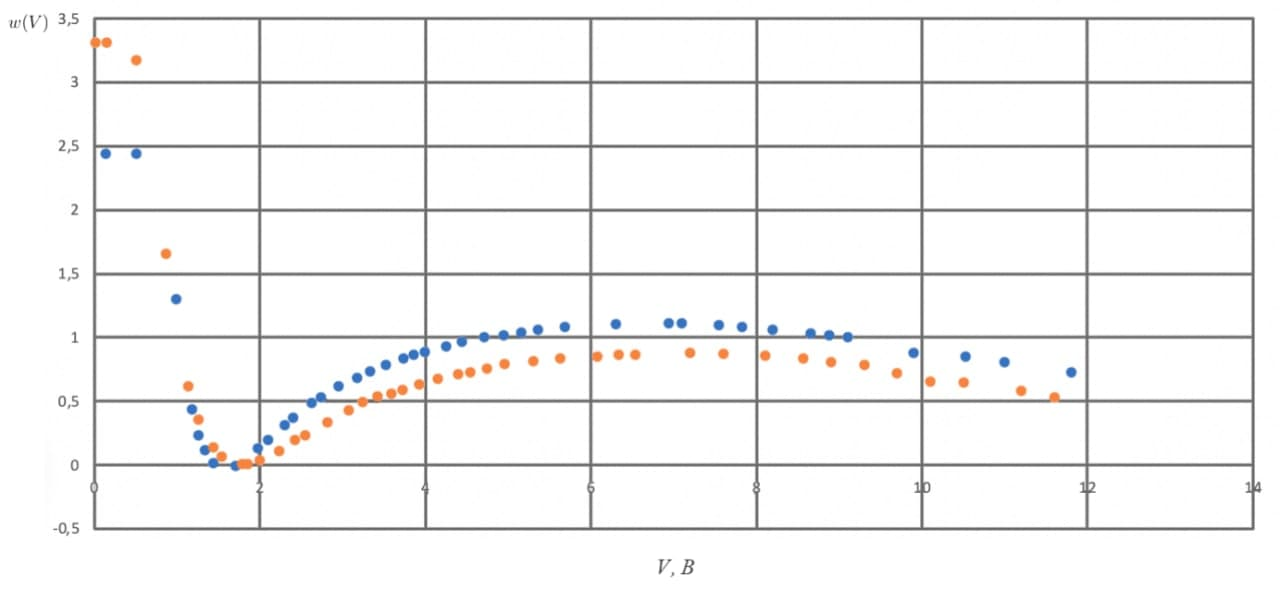
\includegraphics[scale=0.5]{123}

Рисунок 1.
\end{center}

Убедимся в том, что отношение длин волн водородных линий соответствует формуле (2).
\begin{center}
\includegraphics[scale=0.45]{table3.1}
Таблица 3.1.         $\qquad\qquad\qquad\qquad\qquad$  Таблица 3.2.
\end{center}


Значения таблиц совпадают с точностью до третьего знака.

\paragraph*{Изучение молекулярного спектра йода.}

Исследуется спектр поглощения паров йода в видимой области, по результатам измерения вычисляется энергия колебательного кванта молекулы йода и энергия ее диссоциации в основном и возбужденном состояниях.



Занесём в Таблицу 4 положения барабана, для различных линий спектра йода.

Цветам в ней отмечены: самая длинноволновая линия - красная, $h\nu_{1,0}$, шестая по счету от длинноволнового края - жёлтая $h\nu_{1,5}$, граница схождения спектра - фиолетовая, $h\nu_{\text{гр}}$. 

По градуировочной кривой монохроматора определим длины этих трёх линий. Результаты и рассчитанные погрешности занесём в таблицу 5.  

\begin{center}
\includegraphics[scale=0.4]{table5}

Таблица 5.

\includegraphics[scale=0.6]{yod}
\end{center}

Вычислим в электрон-вольтах энергию колебательного кванта возбужденного состояния молекулы йода:
\[h\nu_2 =\frac{h\nu_{1,5} - h\nu_{1, 0}}{5}\]
\[\nu = c / \lambda\]
\[\sigma_{\nu} = \frac{c}{\lambda^2}\cdot \sigma_{\lambda}\]

\[h\nu_2 = \frac{1.925-1.993}{5}=0.013\pm 0.004eV\]

Вычислим энергию электронного перехода $h\nu_{el}$
\[h\nu_{el} = h\nu_{1,0}+h\nu_1 = 1.993+0.027 = 2.020\pm0.003eV\]
Вычислим энергию диссоциации молекулы в основном состоянии $D_1$
\[D_1 = h\nu_{gr} - E_A = 2.456-0.940=1.516\pm0.003eV\]

Вычислим энергию диссоциации молекулы в возбужденном состоянии $D_2$.
\[D_2 = h\nu_{gr} 0 h\nu_{el} = 2.456 - 2.020 = 0.436\pm0.006eV\]

Используя полученные результаты, а также данные о том, что $h\nu_1 = 0.027$эВ - энергия колебательного кванта основного состояния, $E = 0.94$эВ - энергия возбуждения атома,$D_1 = 1.5425$эВ - энергия диссоциации из невозбужденного состояния, $D_2=0.69$эВ - возбужденного состояния.




\begin{center}
\includegraphics[scale=0.8]{table4}

Таблица 4.
\end{center}

\section*{Вывод}
Полученные длины волн серии Бальмера совпадают с теоретическими значениями. Определённое значение постоянной Ридберга совпало с табличным. Были определены различные энергетические уровни молекулы йода.


\end{document} % конец документа

	